\chapter{Large Hadron Collider}
The Large Hadron Collider (LHC) is a two ring superconducting hadron 
accelerator and collider. It is located on the border of Switzerland
and France to the northwest of the metropolitan area of Geneva.
The LHC is installed in a 26.7 km long tunnel which was originally constructed
from 1984 to 1989 for the Large Electron Positron (LEP) collider. 
While a hadron hadron collider does not have the same limitations
due to synchrotron radiation as an electron positron collider, 
the financial benefits of building the LHC in an existing collider tunnel 
provided a strong motivation. 
%The LHC uses superconducting magnets that operate at 2 K
The LHC is designed to collide protons at a center of mass energy of 14 TeV.
The overall purpose of constructing a hadron collider with such a high
center of mass energy is to explore the physics beyond the standard model.  

%The LHC is the product of an international collaboration and funded by a large number of country member states.
%%try not to start every sentence with "THE LHC"
\section{Layout}
A schematic layout of the LHC is shown in figure \ref{fig:LHCring};
the LHC follows the LEP tunnel geometry.
The tunnel is 2.7 m in diameter and houses a twin-bore magnet 
which provides both rings in the same structure.
As can be seen in figure \ref{fig:LHCring},
the LHC can be schematically divided 
into 8 octants. At the center of each octant is a straight section and between
each of the 8 straight section there are 8 arcs. Each straight section
is 528 m long and can serve as an experimental point, where a beam
crossing occurs, or as a utility insertion point.
\begin{figure}[t]
  \centering
	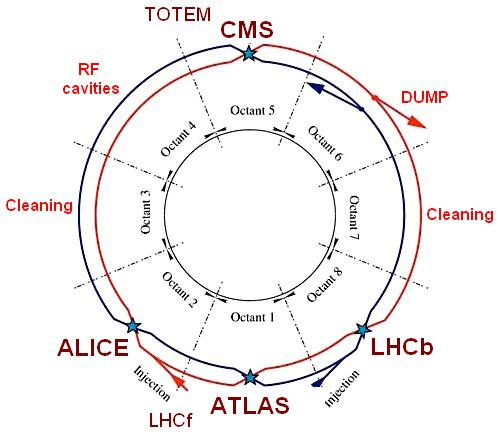
\includegraphics[width=0.6\textwidth]{images/LHCring.jpg}
  	\caption[LHCring]
   	{LHC Experimental and Utility Insertion Layout}
	\label{fig:LHCring}
\end{figure}
The LHC is host to five experiments: ALICE is a dedicated ion
experiment, LHCB is designed to study B-physics,
TOTEM detects protons from elastic scattering at small angles,
and two detectors designed to study a wide range of 
physics processes, CMS and ATLAS.
CMS and ATLAS are both high luminosity experiments;
the ATLAS experiment is located at Point 1 and, on the opposite side
of the ring, CMS is located at Point 5. 
%%some info about LHCb and ALICE
% the LHC-B experiment at Point 2, ALICE experiment is at Point 8. 
Located at points 3 and 7 are collimation systems for beam cleaning,
the beam dump is at point 6 and point 4 houses an RF system for acceleration.

Each of the arcs that stretch between the straight sections
are made of 23 arc cells. Each arc cell is 106.9 m in length
and is comprised of two half cells each of which are 53.45 m long.
A schematic of the interior of the arcs showing the dipole magnets,
cryogenic system and overall layout can be see in figure \ref{LHCdipolemagnets}

\begin{figure}[t]
  \centering
	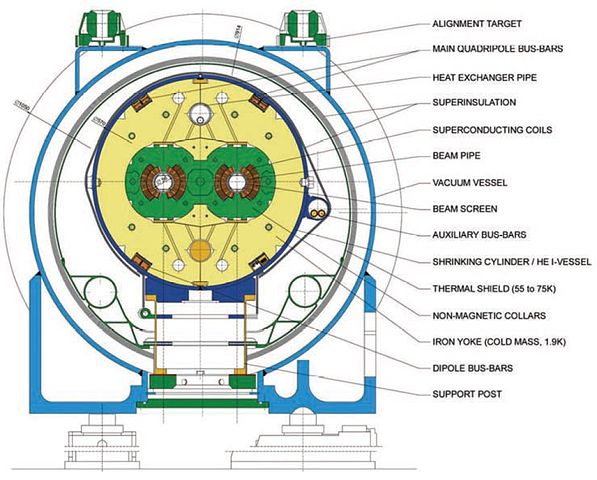
\includegraphics[width=0.6\textwidth]{images/LHCdipolemagnets.jpg}
  	\caption[LHCCell]
   	{Cross section of cryodipole}
	\label{fig:LHCdipolemagnets}
\end{figure}

\section{Performance Goals and Constraints}
The LHC was designed with the purpose of exposing the physics that lies beyond the standard
model. To achieve this, proton collisions must have high energies, 
to explore regions of phase space that 
had remained out of reach at previous particle colliders, and high 
intensities, to search for rare processes.
Considering a process with an event cross section of
 $\sigma_{event}$
the number of events, N, delivered per second as a function
of machine luminosity, L, is,
\begin{equation}
N=L\sigma_{event}.
\end{equation}
The machine luminosity itself depends on optimization of the beam parameters,
\begin{equation}
L=\frac{N_{b}^{2}n_{b}f_{rev}\gamma_{r}}{4\pi \epsilon_{n}\beta*}F
\label{eq:MachineLumi}
\end{equation}
Here, $N_{b}$ is the number of particles per bunch, $n_{b}$
is the number of bunches per beam, $f_{rev}$ is the
revolution frequency, $\gamma_{r}$ is the relativistic factor, 
%$\epsilon_{n}$ is the normalized transverse beam emittance, 
%$\beta^{*}$ is the a function of the collision point fix
and F is the geometric luminosity reduction factor due to the crossing
angle at the collision point. %In addition to intensity loss from collisions, there are also
%losses due to a gradual increase in bunch emittance, $\epsilon_{n}$.
The normalized transverse beam emittance, $\epsilon_{n}$, is a measure of the
beams cross sectional size and $\epsilon_{n}\pi$ is the 
total cross sectional area occupied by beam particles. 
F is the geometric luminosity reduction factor due to the crossing angle
at the interaction point (IP),
\begin{equation}
F=\left(1+\left(\frac{\theta_{c}\sigma_{z}}{2\sigma*}\right)^{2}\right)^{-1/2}.
\label{eq:F}
\end{equation}
In (\ref{eq:F}), $\theta_{c}$ is the full crossing angle at the IP, $\sigma_{z}$ is the
RMS bunch length, and $\sigma*$ is the transverse RMS beam size
at the IP.
A number of factors constrain the luminosity that the LHC is capable
of delivering: %, the most obvious of which is the Luminosity Lifetime.
During nominal operation a decrease in bunch intensity occurs
due to collisions in the IPs.
%Collisions are the primary cause of luminosity lifetime decay during nominal operation.
%is collisions which cause a decrease in bunch intensity.
Initially, the decay time of the bunch intensity is,
\begin{equation}
\tau_{nuclear}=\frac{N_{tot,0}}{L\sigma_{tot}k},
\end{equation}
where $N_{tot,0}$ is the initial beam intensity, L is the initial
luminosity and $\sigma_{tot}$ is the total cross section and 
k the number of IPs.
The luminosity as a function of time is then,
\begin{equation}
L(t)=\frac{L_{0}}{(1+t/\tau_{nuclear})^{2}},
\end{equation}
here, $L_{0}$ is the initial luminosity.
%$\epsilon_{n}$
When accounting for effects due to a gradual increase in
 $\epsilon_{n}$ %and friction between protons and the %%%fix this.... January 9th, read about beam shield
 this results in a net luminosity lifetime of 
\begin{equation}
\tau_{L} = 14.9 h .
\end{equation}
This further implies that it takes only $\approx$10h for the
beam to reach $1/e$ of its initial intensity.

%Finally, it is desired that each of the high luminosity experiments
%are delivered a large amount of integrated luminosity per year. %%don't like this sentence
The maximum total integrated luminosity is then,
per fill is,
\begin{equation}
L_{int}=L_{0}\tau_{L}\left[ 1-e^{-T_{run}/\tau_{L}}\right]
\end{equation}
Another factor which effects the integrated luminosity that can
be delivered per year is turnaround time between fills.
After a fill has been ended it is expected the turnaround time
needed between the end of the fill and the start of a new fill
to be $\approx$7 hours. Therefore, if the machine is operated for 200 days
per year and an optimum run time of 12 hours this leads to a theoretical 
total maximal delivered integrated luminosity per year of 80 fb$^{-1}$
to 120 fb$^{-1}$. The operating conditions for 2011 and 2012
are outlined in section \ref{sec:Conditions}.

%%%fix this:
%A number of factors constrain the luminosity that the LHC is capable
%of delivering: 
Refering to equation (\ref{eq:MachineLumi}) 
$N_{b}/\epsilon_{n}$ is limited by the %%new paragraph?
non-linear beam-beam interaction that occurs when beams collide. This
beam-beam interaction is parameterized by a linear tune shift, $\xi$, 
\begin{equation}
\xi=\frac{N_{b}r_{p}}{4\pi\epsilon_{n}}
\end{equation}
where $r_{p}$ is the classical radius of the proton
and $\epsilon_{n}$ is the beam emittance.
Data from previous hadron colliders show that when summed over
all IPs $\xi$ should not exceed 0.015. %new paragraph?
%Furthermore, the %%% beam width ?? is affected due to
The transverse beam emittance $\epsilon_{n}$ is limited by the 
mechanical aperture of the LHC arcs which is given by the beam screen dimensions.
The beam screen has a height of $2 \times 17.3$ mm and a total width
of $2 \times 22$ mm. In terms of the RMS beam size 
the beam requires a minimum aperture of 10 $\sigma$ this corresponds to a 
nominal beam size of 1.2 mm. Finally, if this is combined with a
peak $\beta$ function of 180 m in the LHC arcs, the maximum acceptable
transverse beam emittance is $\epsilon_{n}=3.75 \mu m$ and a 
maximum bunch intensity of $N_{b}=1.15 \times 10^{11}$.

%Mechanical Aperture
A total beam current of 0.584 A corresponds to a stored energy
of approximately 362 MJ; the LHC magnet system has a stored
electromagnetic energy of more than 1 GJ.
At the end of a fill or in case of a malfunction the stored
energy in the beam needs to be dumped. Therefore, the beam
and magnet dumping systems lead to additional constraints
on the maximum allowed energies and intensities.
%define synchrotron radiation and larmour's formula

Power loss due to synchrotron radiation is given by larmor's formula,
\begin{equation}
P=\frac{\mu_{0}q^{2}a^{2}\gamma^{4}}{6\pi c}
\end{equation}
%While synchrotron radiation due to particle acceleration of protons%%double check all of this, i'm tired
%is smaller than that of electrons 
Where $\mu_{0}$ is vacuum permeability, 
$q$ is the charge of the proton, 
a is the centripetal acceleration, 
and $\gamma=(1-(v/c)^{2})^{-1/2}$.
This puts further requirements on the LHC design as the heat generated in this process and
 from luminosity-induced losses and interaction with a resistive wall 
must be absorbed by the cryogenic system.

In order to collide two counter-rotating proton beams separate magnetic fields
with opposite dipoles are needed. To maintain good operating conditions
the magnets must be identical in field strength. 
Due to the space constraint in the LEP/LHC
tunnel twin bore magnets are used that consist of two sets of 
coils and beam channels within the same structure and
sharing the same cooling. 
The superconducting technology used in the twin bore magnets is at the leading edge.
The magnetic field strength in a solenoid is given by  
\begin{equation}
B=\mu nI
\end{equation}
where $n$ is the number of turns per unit length and $I$ is the current in the winding.
To achieve the strong magnetic field needed for a charged particle collider
a very high current density is needed. 
The high current is achieved using superconducting
metal that has an extremely low resistance.
The current density is then increased by using multiple windings of 
wires. A cable configuration known as Rutherford cables is able to
minimize the self coupling of the wires while providing a higher density
than simply winding or braiding the cables \cite{WilsonSuperCond}.
At the Tevatron, HERA and RHIC experiments, Niobium Titanium (NbTi)
was used in the Rutherford cables and cooled to $\approx$4K. 
%%%EXPLAIN WHAT RUTHERFORD CABLES ARE
The LHC dipole magnets use NbTi in Rutherford cables as well but are cooled
to a temperature of less than 2K. 
This decrease in temperature
by a factor of two allows the dipole magnets to be operated 
at a much higher magnetic field, up to 8T. 
The cooling of the magnetic field is done 
by a cryogenic system that makes use of liquid He. With the lowering of
temperature comes a reduced heat capacity of the cables themselves.
Therefore, the energy deposition threshold that can raise the 
temperature of the windings above their critical temperature and
cause the coil to enter its resistive state (known as a 'quench') is greatly
reduced. To mitigate these issues a tighter control of current movement
and heat dissipation in the cables is required. 
%%In 2008 a during a routine ramp up a quench occurred.
%The quench and successive rapid loss of current
%cause a short in the joint of a busbar. This caused an arc
%which punched through the Helium enclosure and released
%Helium from the cell and with it the Helium from connecting
%cells. No one was injured due to this incident, however, 
%

\section{Operation}
\begin{figure}[t]
  \centering
	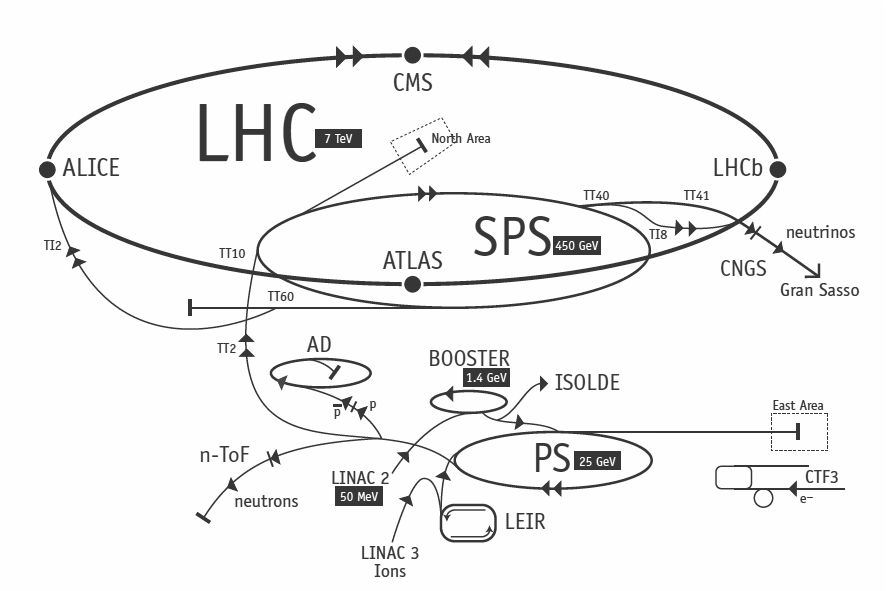
\includegraphics[width=0.75\textwidth]{images/LHCLayout.png}
  	\caption[e/$\gamma$ LHC Layout]
   	{LHC and Experiments Layout}
	\label{fig:LHCRings}
\end{figure}

From their creation in Linear Accelerator 2 until they reached
a final energy per proton of 3.5 TeV (4 TeV) in 2011 (2012),
the proton beams transverse a great distance of accelerator complex %%better word
%before they reach the final LHC energies 
as shown in figure \ref{fig:LHCRings}.%%figure
Initially, hydrogen atoms are stripped of their electrons by passing them
through an electric field. These protons
then undergo their first round of acceleration in Linear Accelerator 2 (LINAC 2).
In LINAC2 the protons are accelerated in conductors which
are alternately charged positive or negative by radiofrequency (RF) cavities;
%that alternate the charge on cylindrical conductors be
this brings the protons up to 50 MeV and forms the initial bunches. 
After this the protons are
fed into the Proton Synchrotron Booster (PSB) which is made up 
of four superimposed synchrotron rings; here the energy
is increased to 1.4 GeV by RF cavities. In
the PSB the beams start to get squeezed and each bunch is 
split into 3. 
Next, they are injected into the Proton
Synchrotron (PS) where they are accelerated to 26 GeV; each
bunch is split into 4 here and, using an 80 MHz RF system,
bunches are shortened so they can fit into the 200 MHz brackets
of the next RF system. Before reaching the LHC, the final
stage of acceleration, takes place in the
Super Proton Synchrotron where they are brought up to 450 GeV.
Finally, the beam is injected into the LHC where protons are ramped
up until they reached a final energy of 3.5 TeV 
in the 2011 run. In the 2012 run the final energy was 4 TeV. 
The operating conditions of the 2011 and 2012 runs are further
detailed in the next section.

\section{Operating Conditions in 2011 and 2012}
\label{sec:Conditions}
\begin{figure}[hb]
  \centering
	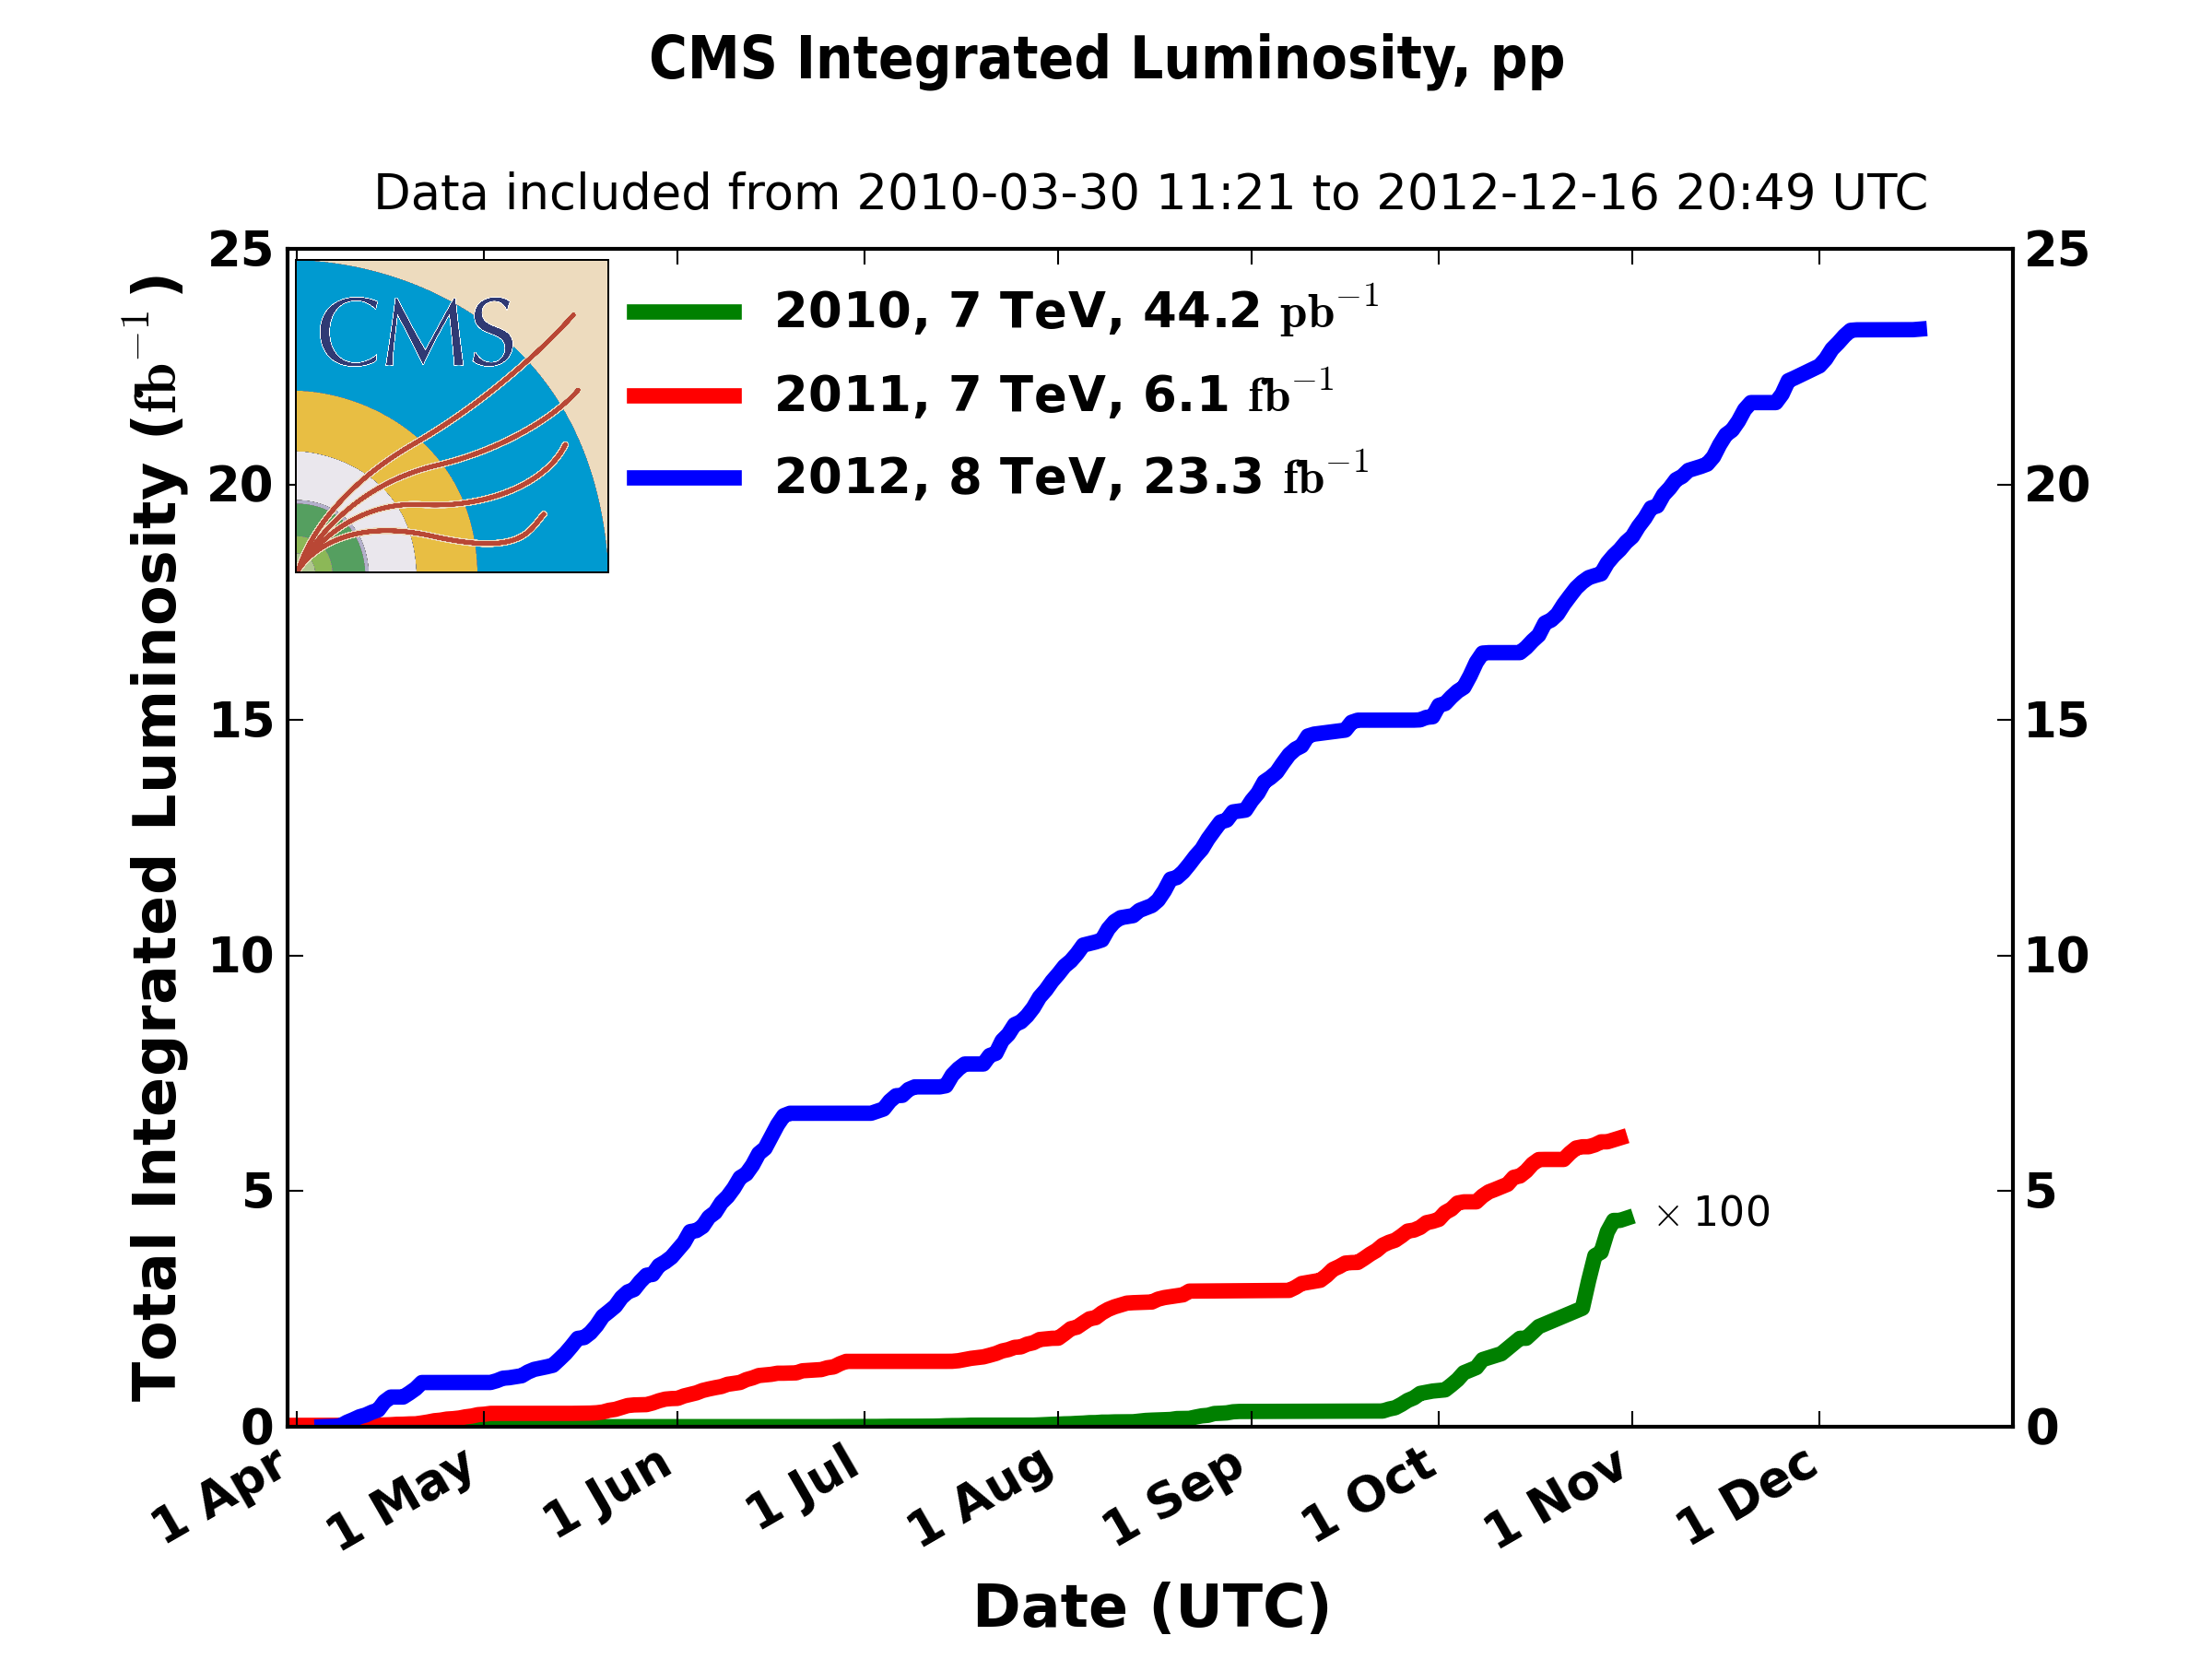
\includegraphics[width=0.5\textwidth]{images/int_lumi_cumulative_pp_2.png}
  	\caption[Total Integrated Luminosity]
   	{CMS Integrated Luminosity}
	\label{fig:deliveredLumi}
\end{figure}
In 2011 the LHC was operated with a center of mass energy of 7 TeV
and a peak luminosity of $2\times10^{33} cm^{-2}s^{-1}$ 
While in 2012 the center of mass energy was 8 TeV and the peak luminosity
was also increased to $7.7\times10^{33} cm^{-2}s^{-1}$.
In both 2011 and 2012 the bunch spacing was 50 ns and the
total number of bunches was 1380. 
The total integrated luminosity delivered by the LHC detector
as a function of time is shown in figure \ref{fig:deliveredLumi}.
%The LHC was designed to operate
%at 14TeV with a peak luminosity of $10^34 cm^{-2}s^{-1}$ and a bunch 
%crossing rate of 25 ns; this scenario is planned for subsequent runs.
%%%finish describing 

%The average event rate is,
%\begin{equation}
%R=L\sigma_{T}
%\end{equation}
%The average rate of events from collisions of a bunch is given by
%\begin{equation}
%N=\frac{R}{R_{B}}
%\end{equation}
%where $R_{B}$ is the LHC crossing rate. 

%\begin{equation}
%\mu=\frac{L\sigma_{T}}{R_{B}f_{B}}
%\end{equation}
%
%The high 